\documentclass[conference]{IEEEtran}
\IEEEoverridecommandlockouts
% The preceding line is only needed to identify funding in the first footnote. If that is unneeded, please comment it out.
%Template version as of 6/27/2024

\usepackage{cite}
\usepackage{amsmath,amssymb,amsfonts}
\usepackage{algorithmic}
\usepackage{graphicx}
\usepackage{textcomp}
\usepackage{xcolor}
\usepackage{bm}
\usepackage{multirow}
\usepackage{tabularx, colortbl, makecell}
\usepackage{etoolbox}

\makeatletter
\patchcmd{\@makecaption}
  {\scshape}
  {}
  {}
  {}
\makeatother

\def\BibTeX{{\rm B\kern-.05em{\sc i\kern-.025em b}\kern-.08em
    T\kern-.1667em\lower.7ex\hbox{E}\kern-.125emX}}
\begin{document}

\title{Target Speaker Extraction using Discrete Representations from 
Self-Supervised Models and Language Models
\thanks{Identify applicable funding agency here. If none, delete this.}
}

\author{\IEEEauthorblockN{1\textsuperscript{st} Beilong Tang}
\IEEEauthorblockA{\textit{Duke Kunshan University} \\
% \textit{name of organization (of Aff.)}\\
Kunshan, China \\
bt132@duke.edu}
\and
\IEEEauthorblockN{2\textsuperscript{nd} Bang Zeng}
\IEEEauthorblockA{\textit{Duke Kunshan University} \\
% \textit{name of organization (of Aff.)}\\
Kunshan, China \\
bangzeng@whu.edu.cn}
% \and
% \IEEEauthorblockN{3\textsuperscript{rd} Zhan Jin}
% \IEEEauthorblockA{\textit{Duke Kunshan University} \\
% Kunshan, China \\
% zhan.jin@whu.edu.cn}
\and
\IEEEauthorblockN{3\textsuperscript{re} Ming Li}
\IEEEauthorblockA{\textit{Duke Kunshan University} \\
% \textit{name of organization (of Aff.)}\\
Kunshan, China \\
ming.li369@dukekunshan.edu.cn}
}

\maketitle

\begin{abstract}
This document is a model and instructions for \LaTeX.
This and the IEEEtran.cls file define the components of your paper [title, text, heads, etc.]. *CRITICAL: Do Not Use Symbols, Special Characters, Footnotes, 
or Math in Paper Title or Abstract. 
\end{abstract}

\begin{IEEEkeywords}
target speaker extraction, speech separation, language models, audio discretization
\end{IEEEkeywords}
\begin{figure*}[t]
    \centering
    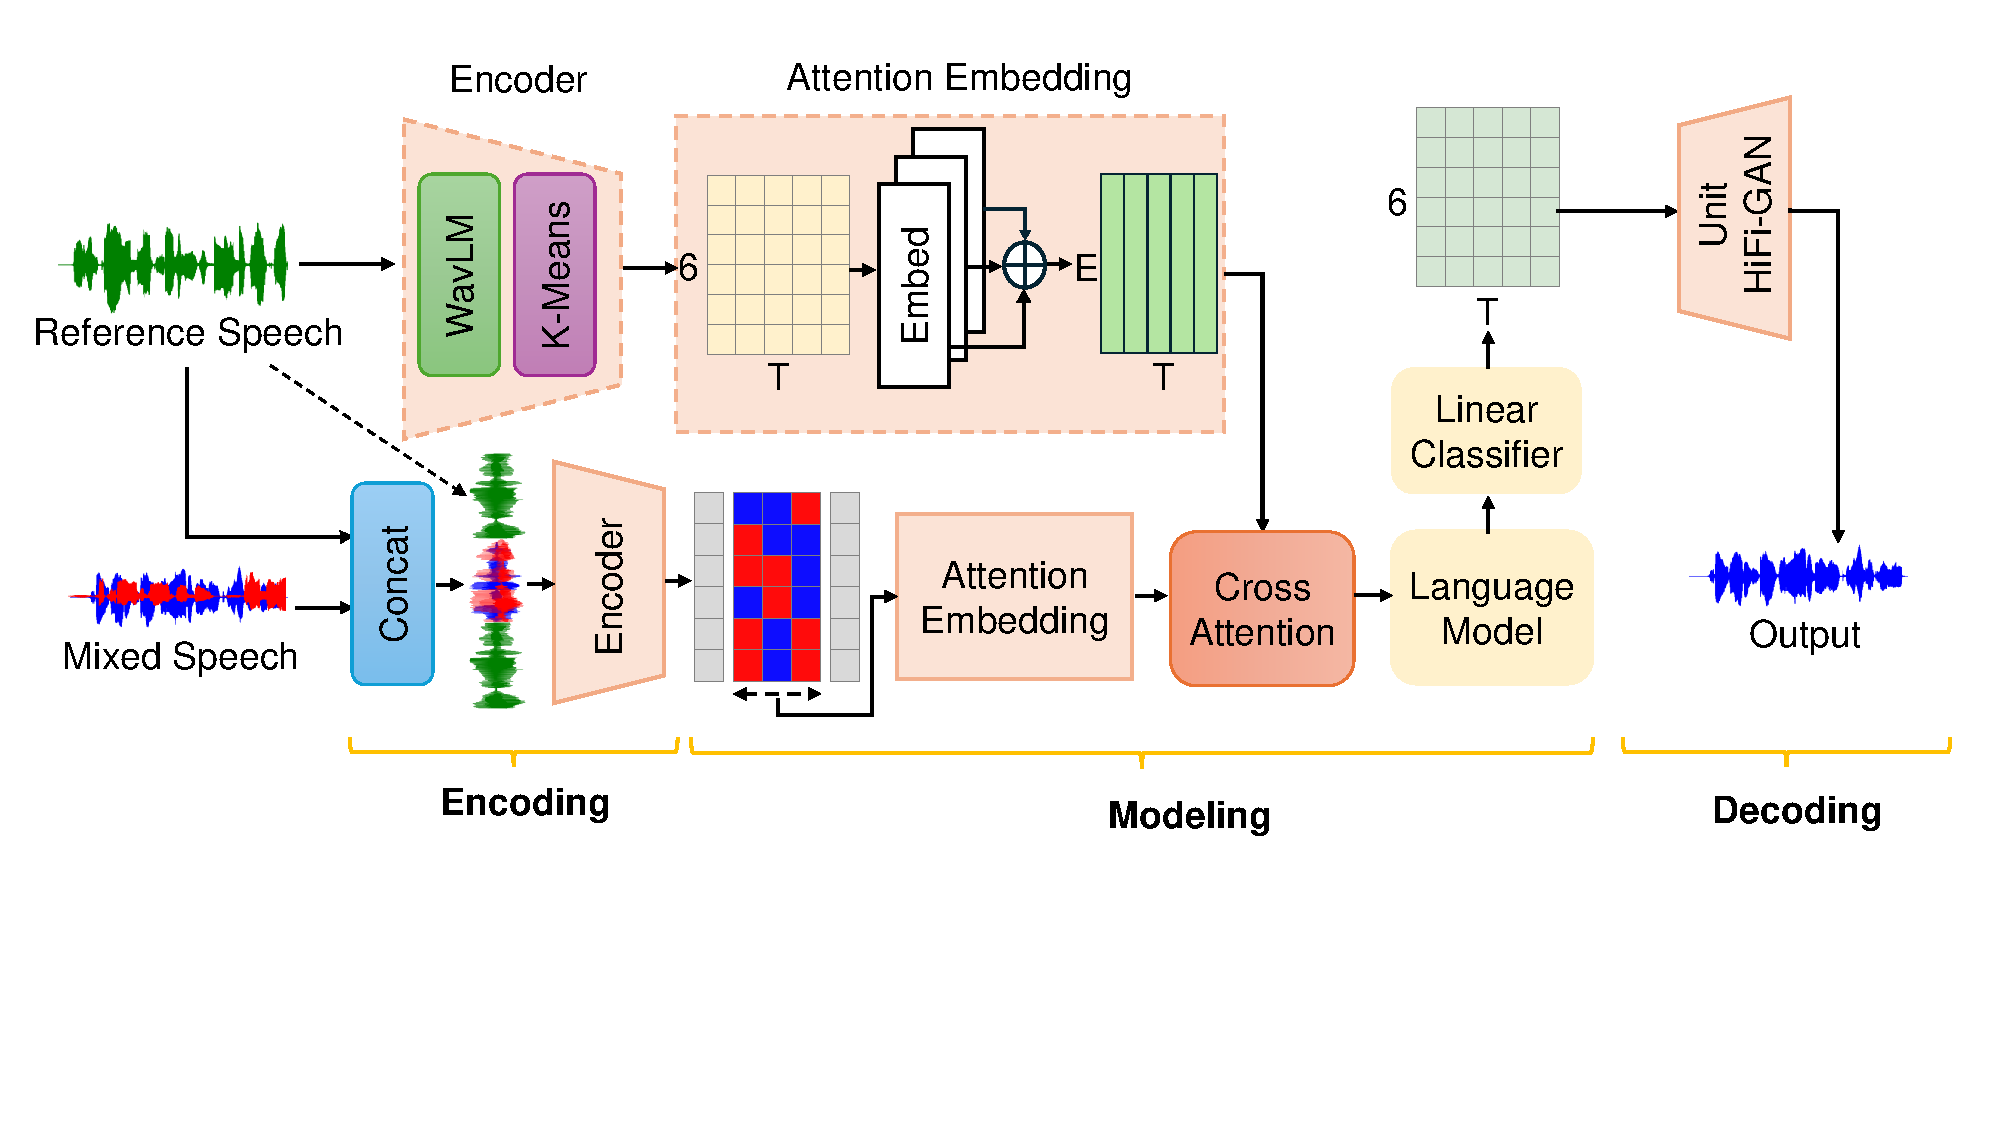
\includegraphics[width=\textwidth]{assets/model.pdf}
    \caption{Overview of TSELM.}
    \label{model}
    \end{figure*}

    \begin{figure}
        \centering
        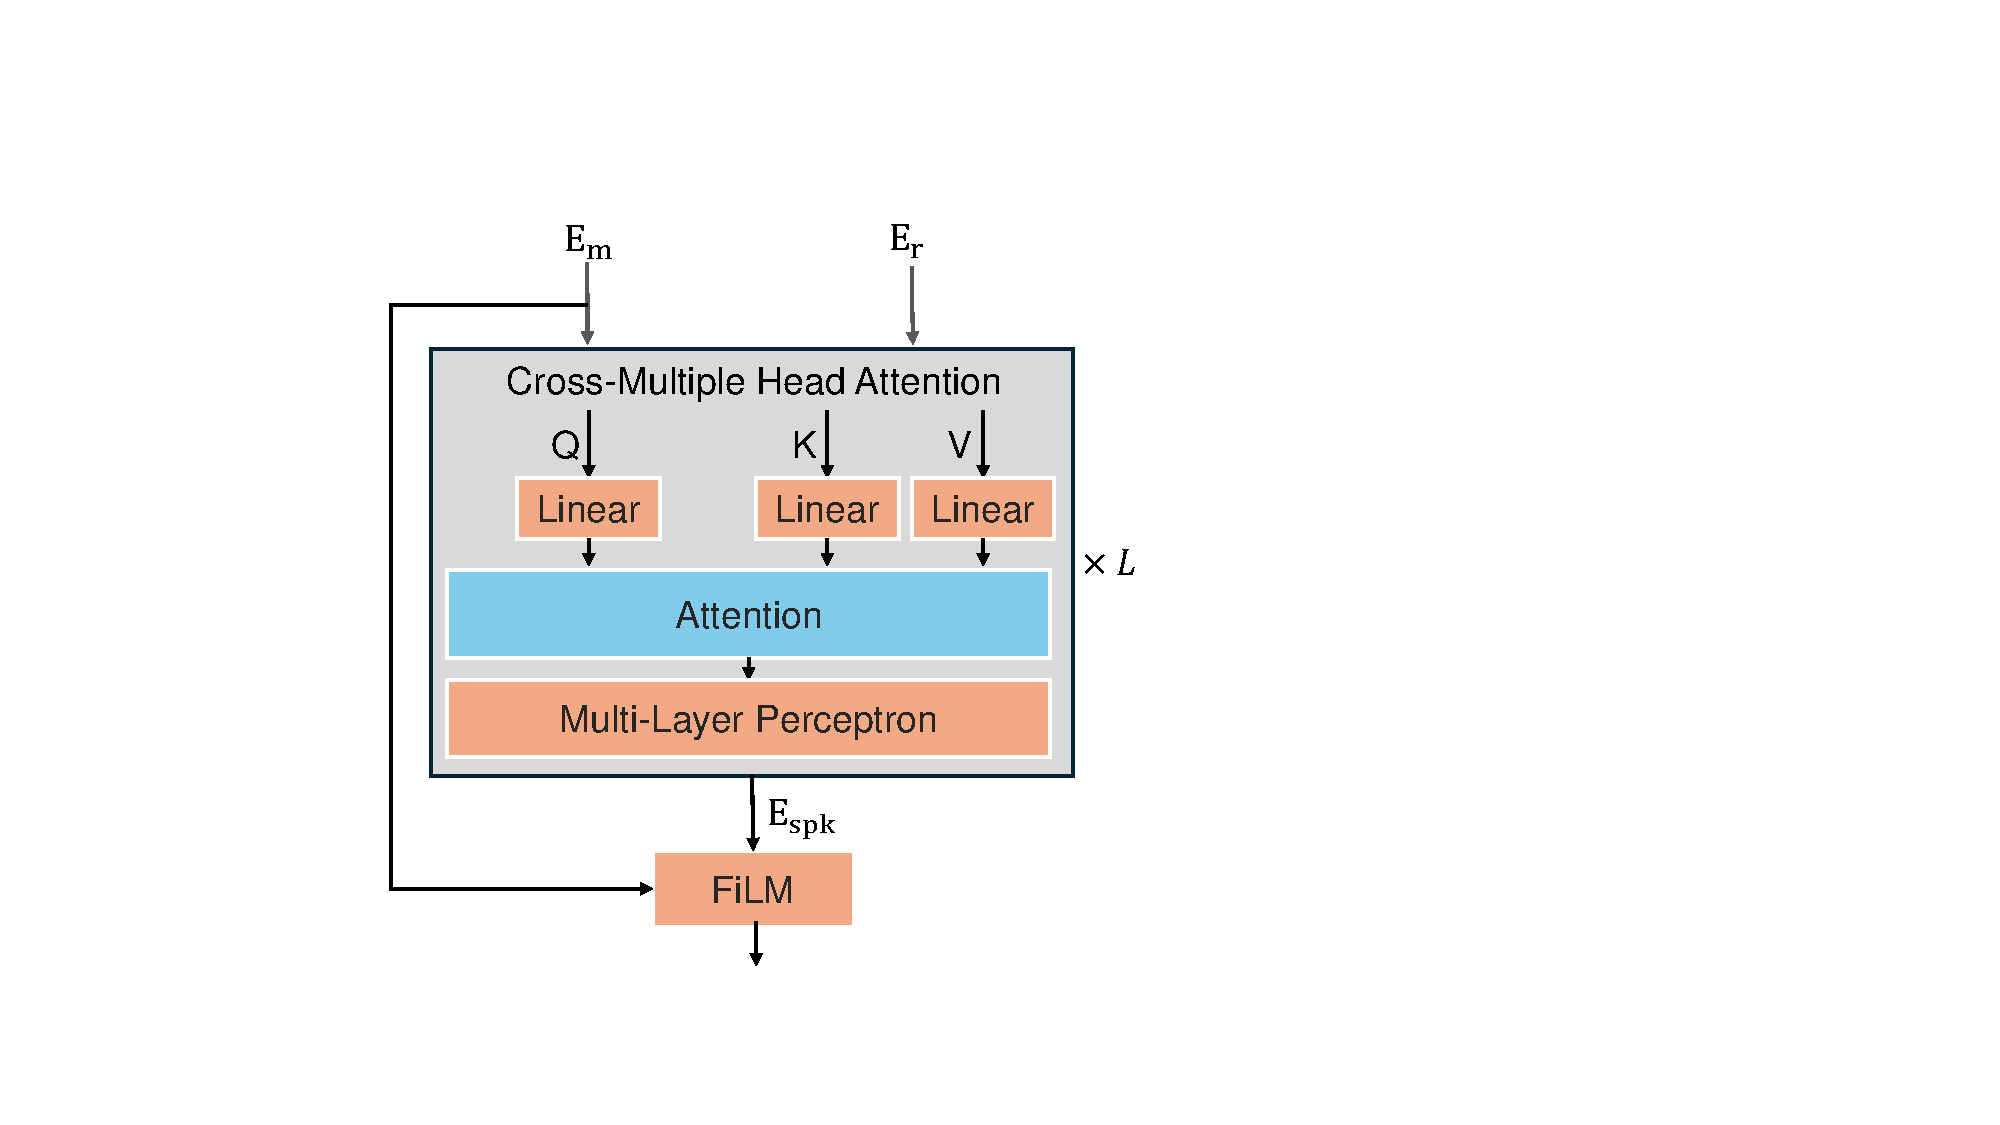
\includegraphics[width=0.35\textwidth]{assets/cross_attention.pdf}
        \caption{Details of Cross Attention mechanism.}
        \label{cross_attention}
        \end{figure}


        
\section{Introduction}
Speech separation, the so-called cocktail party problem \cite{cocktail}, focuses on separating each individual speaker's source from a mixture with multiple speakers. This task is easy for humans but not for computers. 
In real life, speech signals are usually companied with background noise or other speakers' speeches. 
These corrupted signals may not be optimal for tasks like speaker verification \cite{rao2019targetspeakerextractionoverlapped,9414017}, and speech recognition \cite{molkov2017SpeakerAwareNN, 8462661}, emphasizing the importance of having good and robust 
speech separation models.

Unlike blind speech separation, which focuses on separating each utterance from a mixture 
of known speakers, target speaker extraction aims at only extracting the 
target speaker's voice given another auxiliary information of the target speaker. Due to the 
development of Deep Neural Network (DNN), many models nowadays are discriminative models. They 
utilize a masking strategy to minimize the distance between the clean speech and estimated 
speech directly \cite{luo2019conv,spex_plus,sepformer,sef_net}. However, these discriminative 
models may not generalize well to unseen data and might even introduce unwanted distortions \cite{distortion}. To solve these issues, researchers have proposed generative models. This method aims to learn the underlying distribution of the target speaker's voice and use this knowledge to generate the clean speech of the target speaker from a mixture of voices rather 
than directly mapping from mixed speech to clean speech. Some generative models, like diffusion
models \cite{target_diff} and variational autoencoders (VAE) \cite{vae} have been studied. It has been demonstrated that generative models can achieve results comparable to those of discriminative models \cite{target_diff,tokensplit}.

Discretization of audio has been studied due to the advancement of language models (LM). 
This approach translates the audio into discrete tokens simulating text vocabularies and uses LMs to 
model them. This approach simplifies audio generation tasks by transforming the complex 
regression problems into classification problems \cite{dasb}. There are currently two approaches for
audio discretization, the first one uses neural audio codecs \cite{dac}. This approach 
typically captures the acoustic features of the audio \cite{speech_tokenizer}. The second approach 
utilizes  self-supervised Learning (SSL) models like HuBERT \cite{hubert} and WavLM \cite{wavlm}.
SSL models have demonstrated 
excellent performances on many downstream tasks \cite{superb}. These SSL models extract  
continuous representations containing rich semantic and timbre information from a given speech. 
As demonstrated in \cite{dasb}, SSL models perform better than audio codec in tasks like speech 
enhancement and speech separation. Therefore, in this 
paper, we mainly explore the discretization of SSL models.  

Discretization methods have been studied for speech 
enhancement \cite{selm} and blind speech separation \cite{dasb,tokensplit}, 
however, this approach has 
been rarely studied for target speaker extraction. In this paper, we present a novel way to do 
target speaker extraction using discrete tokens and LMs (TSELM). Inspired by the blind speech separation 
networks proposed in DASB \cite{dasb}, our model has three stages: encoding, modeling and decoding.
For the encoding stage, reference speech and mixed speech are tokenized using WavLM and 
Kmeans as tokenizer. Unlike SELM \cite{selm}, which uses the 6th layer of WavLM as input to the Kmeans layer, 
we follow the recipes in \cite{dasb} and uses the output from hidden 
layers 1, 3, 7, 12, 18, 23 of WavLM as input to the Kmeans layer. 6 Kmeans models
are trained and applied on each layer output respectively. 
Our results indicate that using multiple layers as 
input is better 
than using only the 6th layer. The reference speech is fed to the encoder directly. 
However, for the mixed speech, instead of directly passing it to the WavLM model, we first concatenated the reference speech on both sides 
of it before passing. After tokenization, we use only the tokens 
corresponding to the mixed speech. For the modeling stage, we utilized an attention 
embedding mechanism to add each embeddings of all layers together. We used a Cross 
Attention mechanism similar in \cite{sef_net} to inject the speaker information. 
An encoder-only LM, following by a linear classifier, is applied after the cross attention module
to output the reconstructed tokens. 
For the decoding stage, we used the pretrained unit HiFi-GAN 
in \cite{unit_hifi} to reconstruct the 
discrete tokens back to audio. Unlike SELM \cite{selm}, where a conformer 
detokenizer is trained 
to reconstruct the WavLM embeddings using Kmeans center embeddings before HiFi-GAN, \cite{unit_hifi} has proposed a scalable HiFi-GAN using dropout mechanism to directly 
reconstruct audio from multiple layers of tokens without a conformer detokenizer. It 
has also eliminated the trouble of training a HiFi-GAN for each layer. The encoder and 
decoder is freezed during the training. The model overview is in Fig.\ref{model}. 
Through extensive studies, we have demonstrated this method has achieved comparable results in terms 
of speech quality and intelligibility. To the best of our knowledge, we are the first to explore 
using discrete tokens to conduct target speaker extraction.



\section{Method}
Our model consists of three stages: encoding, modeling, and decoding. The encoder and decoder are 
pretrained models and they are freezed during training. For the encoding stage, we use multiple layers of WavLM 
and publicly available Kmeans 
models in \cite{dasb} to produce the discretized tokens. We use a special concatenation 
strategy to encode the mixture speech. For decoders, we use the scalable HiFi-GAN available in 
\cite{dasb} to reconstruct the audio from discretized tokens. Our main focus is on the
modeling stage. We apply an attention embedding mechanism to embed discrete tokens from different 
layers into one single embedding. Encoder-only LM and linear classifier is applied afterwards to optimize the likelihood of probability 
distribution of the clean tokens. 


\subsection{Encoding}


\begin{table*}
    \setlength{\tabcolsep}{12pt} % Adjust column spacing
    \renewcommand{\arraystretch}{1.3}
    \begin{center}
        \begin{tabular}{ccccccccc}
            \Xhline{2\arrayrulewidth} % Bold top line
            \multirow{2}{*}{System} & \multirow{2}{*}{Category} & \multirow{2}{*}{Model type} & \multirow{2}{*}{Model size} & \multicolumn{3}{c}{ DNSMOS $\uparrow$} & \multirow{2}{*}{dWER $\downarrow$} & \multirow{2}{*}{Spk Sim $\uparrow$} \\
            \cline{5-7}
              &                   &                             &                             & SIG     & BAK     & OVL    &                       &                          \\ 
            \hline
            Mixture                 & - & -                           & -                           & 3.39    & 3.14    & 2.68   & 79.3\%                & -                        \\
            Target-discrete-WavLM   & G & -                          & 330M                           & 3.57    & 4.10    & 3.32   & 11.3\%                & 0.653                    \\
            \hline
            Spex+                   &  D & Continuous                  & 11M                         & 3.36    & 3.76    & 2.98   & 19.3\%                & 0.923                    \\
            \hline
            Continuous-WavLM   & G    & Continuous                  & 220M                        & 3.56    & 4.06    & 3.27   & 14.7\%                & 0.877                    \\
            TSELM-L-Hybrid    & G       & Hybrid                      & 468M                        & 3.50    & 4.06    & 3.22   & 19.8\%                & 0.924\_d                 \\
            TSELM-S-NoConcat           & G       & Discrete                    & 354M                        & 3.47    & 4.03    & 3.19   & 69.6\%                & 0.868\_d                 \\
            \hline
            TSELM-S           & G       & Discrete                    & 354M                        & 3.50    & 4.07    & 3.24   & 28.1\%                & 0.892\_d                 \\
            TSELM-M          & G        & Discrete                    & 389M                        & 3.49    & 4.05    & 3.22   & 28.4\%                & 0.901\_d                 \\
            TSELM-L         & G         & Discrete                    & 468M                        & 3.49    & 4.05    & 3.22   & 27.1\%                & 0.905\_d \\
            \Xhline{2\arrayrulewidth} % Bold top line              
            \end{tabular}
            \linebreak
            \caption{The performance of different systems on Libri2Mix testset. For TSELM-L-Hybrid  
            and TSELM, we compare the speaker similarity with the discretized target speech 
            (Target-discrete-WavLM) instead of the target speech due to the observation that 
            the process of discretization already losses the speaker information (0.653 for 
            Target-discrete-WavLM). We use "\_d" to denote it.  }
            \label{main_exp}
      \end{center}
  \end{table*}

We use pretrained SSL model WavLM Large \cite{wavlm} to 
encode the speech into continuous representations. We use the output from 6 hidden 
layers 1, 3, 7, 12, 18, 23. Given a speech signal \(s \in R^{T'} \), the output 
of WavLM will be a tensor \(\bm{r}\) of shape \(n \times T \times E\) where 
\(n\) specifies the number 
of output layers (6 in this case), and  \(T\) is the time 
dimension and \(E\) stands for the 
embedding dimension, specifically 1024 in WavLM Large. The Kmeans tokenizer uses \(n\) numbers of  Kmeans model 
separately on each output layer. Each model uses the same clustering number denoted by \(K\).
After tokenization, the continuous embedding \(\bm{r}\) will be transformed to a tensor \(\bm{d}\) of shape \(n \times T\) where each value \(\bm{d}_{(n_i,t)} \in (0, K-1), n_i \in (0,n), t \in 
(0, T)\). We choose \(K\) to be 1000 in our experiments. For reference speech and mixed speech, we 
use the same Kmeans model and the same layer output of WavLM. The encoder is freezed during training.

The encoding strategy on the mixed speech plays a pivotal role in the model performance. Assume we 
have a reference speech \(s_r \in R^{T^r} \) and mixed speech \(s \in R^{T'}\). 
We follow the 
aforementioned procedure for 
reference speech to get tensor \(\bm{d_r}\) of shape \(n \times T_r\). But for the mixed 
speech, instead of directly following the procedure, we first concatenate it with 
the reference speech to get \(s' = [s_r, s_m, s_r] \in R^{(T^r+T'+T^r)}\). Then we use this speech 
as input for the encoder, obtaining output \(\bm{d'}\) of shape \(n \times (T_r+T+T_r)\) where \(T\) 
denotes the length of output by directly passing the mixed speech without concatenation. \(\bm{d'}\) 
contains the discrete tokens for two pieces of the same reference speech and one piece of the mixed 
speech, we select tensor \(\bm{d}\) belonging only to the mixed speech of shape \(n\times T\) as the 
encoder output. This process is inspired by the training schema of WavLM \cite{wavlm}. To ensure the 
model correctly outputs rich information of the target speaker, it is trained by 
having a clean speech overlapped with another interference less than 50\% of the length of the clean 
speech and using the first utterance as the main speaker. By this way, the model identifiers the 
main speaker and produces embedding focusing on the main speaker. Our later experiments showed that 
this strategy plays an important role in the model performance. 



\subsection{Modeling}
\subsubsection{Attention Embedding}
After obtaining the discrete tensor \(\bm{d}\) with shape \(n\times T\), we use 6
learnable embedding tables each with \(K\) entires to embed the 6 layers 
respectively, each resulting in a tensor of shape \(T \times E\). 
After embedding, we follow the same recipe as in \cite{dasb} to 
aggregate the tensor by using attention mechanism to sum all the 6 tensors. This summation 
keeps the information of each layer while reducing the system complexity by reducing the 
dimension of layers. After attention embedding, we obtain reference embedding \(E_r\) and 
mixture embedding \(E_m\).

\subsubsection{Cross Attention}
One of the key factors in target speaker extraction is to 
inject the information of target speaker 
into the mixture. Spex+ \cite{spex_plus} jointly trains a speaker verification task module 
besides the separator, which might not be optimal for the separator task \cite{sef_net}. SEF-Net \cite{sef_net} has proposed an speaker embedding free way to inject the 
target speaker information into the mixture by using cross attention module, and it has 
achieved superior performance compared to other methods. Therefore, we apply 
the cross attention module to inject the reference embedding into the mixture. The details 
are in Fig.\ref{cross_attention}.
The cross attention module consists of a stack of cross-multiple head attention modules, 
and a FiLM module. 
We use \(E_m\) as query and \(E_r\) as key and value for 
the attention module. The output of the cross-multiple head attention module \(E_{spk}\)
is passed together with \(E_m\) to the feature-wise linear modulation (FiLM) get the final output of the module. The output of 
FiLM is denoted as \(E_f = FiLM(E_m, E_{spk}) = \gamma E_{spk} \cdot E_m  + \beta E_{spk} \) where 
\(\gamma\) and \(\beta\) are learnable parameters denoting the scaling and shifting vectors 
respectively. The output is then fed to the language model for later modeling.  
\subsubsection{Language Modeling}
We use encoder-only language models containing multiple self-attention modules to model the injected 
embedding \(E_f\). Due to encoder-only style, the LM is able to learn from all the positions. 
Finally, 6 linear classifiers each with dimension \(K\) is used to produce the probability 
distribution of each layer respectively.
Cross-entropy loss is applied between 
the output tokens and the clean tokens through discretizing the 
ground truth clean audio. 

\section{Experiments}

\subsection{Training}

We use the publicly available Kmeans tokenizer and scalable 
HiFi-GAN decoder in \cite{speechbrain}. The Kmeans tokenizer
is trained on \texttt{train\_clean\_100}, \texttt{train\_clean\_360}, and \texttt{train\_other\_500} of
LibriSpeech \cite{librispeech}, and the scalable HiFi-GAN is trained on \texttt{train\_clean\_100} of 
LibriTTS \cite{libritts}. The modeling stage is trained on 
\texttt{train\_clean\_100} and \texttt{train\_clean\_360} of LibriSpeech. All training data are 
generated on the fly with relative SNR between 0 dB to 5 dB. The mixture audio is segmented to 3 
seconds and the reference speech is segmented to 4 seconds. 

We use the output from hidden layers 1, 3, 7, 12, 18, 23 from WavLM Large and Kmeans model with 
\(K=1000\).
We use embedding dimension 1024,  4 transformer 
encoders each with 16 heads and MLP with hidden dimension of 1024 in the cross attention module. We 
use layer norm after the cross attention module. 
We use separate embedding tables in attention embedding module for reference and mixed speech due to our observations that not 
sharing embeddings does slightly better than sharing embeddings. The LM of small version TSELM-S uses 
embedding dimension \(d\) = 256, absolute sinusoidal positional embedding, conformer encoders as backbone of LM. The conformer encoder is composed of 
6 layers with kernel size 31 each with 4 heads and an MLP with hidden dimension 2048. The medium version TSELM-M uses \(d\) = 512 with 8 layers and 8 heads and the large version TSELM-L uses 
\(d\) = 768 with 12 layers and 16 heads. We use AdamW as 
our optimizer for all the experiments. The learning rate 
is \(5 \times 10^{-4}\) for TSELM-S and \(5 \times 10^{-5}\) for TSELM-M and TSELM-L. We use 8 16Gb ram GPUs. Our batch size is set to 128. We train the model for 40k steps. 


\subsection{Evaluation}
We use the \texttt{dev} set of Libri2Mix \cite{librimix} to test our model performance and compare it with 
other baseline models. 

It is shown that metrics like PESQ, SI-SNR, STOI do not reflect speech quality of output of 
vocoders due to the fact that the vocoder output does not focus strictly on frame alignment
\cite{tokensplit,selm}. We used DNSMOS \cite{dnsmos} to measure the speech quality, and differential 
word error 
rate (dWER) \cite{dwer} to measure the speech intelligibility. For speaker similarity, we use the 
public WeSpeaker \cite{wespeaker}.


\subsection{Baseline models}
All models are reflected in Table \ref{main_exp}. 
TSELM is compared with Spex+, a discriminative separation model \cite{spex_plus} trained on Libri2Mix \cite{librimix}. Since the discretization might lose some 
speaker information compared with continuous methods. We compare the speaker 
similarity of TSELM with the target audio produced by discretizing the clean audio, which is denoted by Target-discrete-WavLM, and it is the upper bound of our model  
performance. Besides TSELM, we did two experiments 
denoted by Continuous-WavLM and TSELM-L-Hybrid using the same training data. 
For Continuous-WavLM, we directly
passed the embeddings of the 6th hidden layer output of WavLM to the cross attention  
and LM. Concatenation strategy is stilled applied to the mixed speech. Mean Square Error loss is applied between the output embeddings and the clean 
embeddings. We use the HiFi-GAN in \cite{knn_vc} to reconstruct the audio. For 
TSELM-L-Hybrid, inspired by MaskSR \cite{mask_sr}, we kept discretizing the reference 
speech while utilizing the continuous embeddings from the reference speech. We call 
it hybrid instead of fully discretized because the mixture speech has continuous 
features instead of discrete features. 

\section{Results and Discussions}
Table \ref{main_exp} shows the performance of different systems on the Libri2Mix test.
The model size for Target-discrete-WavLM denotes the model size of the encoder and 
decoder, which is WavLM Large and HiFi-GAN respectively. DNSMOS is calculated over the 
test sets since it is reference-free. dWER is calculated with the clean speech instead 
of the discretized speech due to our observations that this does not make much difference. 
For TSELM-L-Hybrid and TSELM, we compute the speaker similarity with the discretized
target speech (Target-discrete-WavLM) instead of the target speech.
% due to the observation that the process of discretization already losses the speaker
% information (0.653 for Target-discrete-WavLM). 
We observe that the process of discretization already losses the speaker
information (0.653 for Target-discrete-WavLM), and it might be related to the inevitable speaker 
information loss by the process of discretization. Future work should focus on developing better 
tokenization methods for SSL models. 
Since work focuses on using the discretized information 
to do target speaker extraction instead of developing better tokenization methods, we think it is 
reasonable to compare our outputs with the discretized speech since it serves as an upper bond.   

We observe that our model performs better than Spex+ in terms of the DNSMOS scores but worse in dWER. 
This suggests that our model has better speech quality compared with discriminative models but 
worse in speech intelligibility. One possible reason might be related 
to the discretization process on the mixture 
speech. Our Kmeans algorithm is trained on clean speech instead of mixed speech. 
For speech enhancement, this might be 
good because the level of noise will usually be smaller than the speech. Kmeans might achieve the 
effect of denoising. Discretization on the mixed
speech, however, might cause the output to focus on wrong speakers. 
Our results from TSELM-L-Hybrid 
support 
this. For TSELM-L-Hybrid, we use the continuous embeddings from the mixture speech without discretizing, and it has 
achieved similar dWER with Spex+. Another reason might be related to LM. Right now our encoder-only 
LM satisfies roughly 50\% accuracy. We think using auto-regressive or masking models will achieve 
better results. 

We observe significant dWER increasing without concatenating the reference audio to the mixture, 
as shown 
the TSELM-S-NoConcat in Table \ref{main_exp}. WavLM \cite{wavlm} is demonstrated to have target speaker 
separation capability. The input audio should have the mixture less than 50\% and have the first utterance as target speaker. The output will be a coarse denoised embedding emphasizing the target speaker. 
If the whole input is mixture, we have found that WavLM sometimes will 
extract the wrong speaker. Inspired by SELM's \cite{selm} success in speech denoising. Our pipeline is trying to transform
the target speaker separation problem to speech enhancement problem by using WavLM's denoising capability.









\section*{Acknowledgment}

We want to thank for Kunshan Super Computing SCNet for providing the computing resources. 

\bibliographystyle{IEEEtran}
\bibliography{references}


\end{document}
